\subsection{IDE integration (Introduction by Philipp Haller)}

As the participants of the use-case study were divided into two groups, the first group dealt with the IDE integration of the Pacman simulator after being instructed by an EMA professional.
After successful integration this first group wrote a step-by-step instruction list. The second group used this list to integrate the Supermario simulator into the IDE. Details are given in the following.

\subsubsection{Integration at the example of Pacman (by Malte Heithoff)}
\begin{figure}
	\caption{Main options for the Pacman project in the ide}
	\label{fig:idePacmanTop}
	\centering
	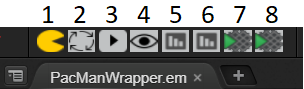
\includegraphics[scale=0.55]{pictures/IDE/IDETop.png}
\end{figure}
To integrate a simulator into the EmbeddedMontiArcStudio several steps were necessary. In figure. \ref{fig:idePacmanTop} you can see the top view of the EmbeddedMontiArc's ide. The five added features here are as follows:
\begin{itemize}
	\item[1.] Open a new tab where you can play a normal game of Pacman
	\item[2.] Generate the WebAssembly of the main component
	\item[3.] Open a new tab in which the simulation of the component takes place
	\item[4.] Generates the visualization of the main component and shows it in a new tab
	\item[5.] Generates the reporting of all components and shows it in a new tab
	\item[6.] Generates the reporting of all components with stream test results and shows it in a new tab
	\item[7.] Run all tests in the repository and show their results
	\item[8.] Run a single test and show its result
\end{itemize}
The features needed to be implemented properly in different places in order to work along the logic of the ide. Each one calls a batch script which again runs the jar for the demanded task for the specific files. In addition, for feature 1 and 2 extra plugins were required which got implemented by the expert group Pacman and could be reused for Supermario.